\section{Projektmanagement}
\subsection{Grundlagen}

\subsubsection{Definition eines Projektes}
Ein Projekt ist ein zeitlich beschränktes Vorhaben zur Erzeugung eines einmaligen Produktes oder Dienstes. 

\subsubsection{Definition des Projektmanagement}
Das Projektmanagement bezeichnet die Gesamtheit von Führungsaufgaben, -organisation, -techniken und -mitteln für die Initiierung, Definition, Planung, Steuerung und den Abschluss von Projekten. 

\begin{multicols}{2}
	\subsubsection{Merkmale eines Projektes}
	\begin{itemize}
		\item einmaliges Vorhaben
		\item klare Ziele
		\item hat Risiken
		\item zeitlich begrenzt
		\item Kostenrahmen
		\item hat innovativen Charakter
		\item es arbeiten mehrere Personen daran
		\item hat Projektleiter \& Projektteam 
	\end{itemize} 
	
	\subsubsection{Kategorien von Projekten}
	\begin{itemize}
		\item Forschungs- und Entwicklungsprojekte
		\begin{itemize}
			\item  Entwicklung neuer Produkte
			\item  Erstellung von Software
		\end{itemize}			 
		\item Investitionsprojekte
		\begin{itemize}
			\item Bau eines Flughafen			
		\end{itemize}
		\item Organisationsprojekte
		\begin{itemize}
			\item Einführung Software
			\item Vorbereitung Veranstaltung
		\end{itemize}
	\end{itemize}
\end{multicols}

\subsubsection{Die 3 Eckpfeiler eines Projektes}
\begin{minipage}{10cm}
	Diese drei Grössen sind voneinander abhängig und sind auch bekannt als \textit{"Fast, Good, Cheap"}
	\begin{itemize}
		\item Ergebnis \textit{\"{}Scope\"{}} $\rightarrow$ Spezifikation
		\item Zeit \textit{"Time"} $\rightarrow$ Terminplan
		\item Aufwand \textit{"Cost"} $\rightarrow$ Budget
	\end{itemize}
\end{minipage}
\begin{minipage}{3cm}
	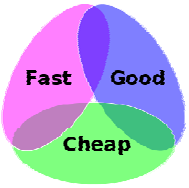
\includegraphics[width=3cm]{images/eckpfeiler.png}
\end{minipage}
\begin{minipage}{3cm}
	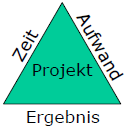
\includegraphics[width=3cm]{images/dreieck.png}
\end{minipage}

\subsubsection{Das Projektdreieck (Magisches Dreieck)}
\begin{minipage}{15cm}
	Diese drei Grössen werden als Dreieck dargestellt. Die Aufgabe des Projektmanagement ist es, ein sinnvolles Verhältnis dieser 3 herzustellen und während der Projektdauer zu gewährleisten. 
\end{minipage}

\subsubsection{Projektbeteiligten (Stakeholder)}
\begin{itemize}
	\item Auftraggeber $\rightarrow$ bezahlt \& befiehlt
	\item Projektleiter (PL) $\rightarrow$ Primär Manager, weniger Fachexperte
	\item Projektmitarbeiter (Projektteam) $\rightarrow$ Fachexperten, hohe Methoden und Sozialkompetenz
\end{itemize}

\subsubsection{Projektorganisationsformen}
\begin{multicols}{3}
	\begin{itemize}
		\item \textbf{Reine Projektorganisation}
		\begin{itemize}
			\item Projektleiter \& Projektteam arbeiten Vollzeit am Projekt
			\item Mitarbeiter sind voll\-kommen dem Projektleiter \newline unterstellt
			\item eher selten
		\end{itemize}
		\item \textbf{Matrix-Projektorganisation}
		\begin{itemize}
			\item Mitarbeiter aus spezif. \newline Bereichen arbeiten nur zeitweise am Projekt mit
			\item Verantwortung ist aufgeteilt zwischen Projektleiter/Linieninstanzen
			\item Häufigste Form
		\end{itemize}
		\item \textbf{Stabs-Projektorganisation}
		\begin{itemize}
			\item Hierarchie ist unverändert
			\item ergänzt durch Projektkoordinator hat keine \newline Weisungsbefugnisse
			\item stimmt Zusammenarbeit mit Mitarbeiter ab
		\end{itemize}
	\end{itemize}
\end{multicols}

\subsection{Projektablauf}
Jedes Projekt hat ein Anfang und ein Ende (Lebenszyklus). Der \textcolor{blue}{vorzeitige Abbruch} ist ein Unfall, ein sogenanntes \newline \textcolor{blue}{ungeplantes} Ende. Jedes Projekt besteht aus 4 Phasen. Die 4 Phasen überlappen sich und laufen parallel ab. \newline Während der Durchführung ist auch die Planung anzupassen. \\
\\
\begin{minipage}{8cm}
	\textbf{Projektphasen:}
	\begin{enumerate}
		\item Projektdefinition
        \subitem (Vorphase, Projektvorbereitung)
		\item Projektplanung
		\item Projektdurchführung
		\item Projektabschluss
	\end{enumerate}
\end{minipage}
\begin{minipage}{8cm}
	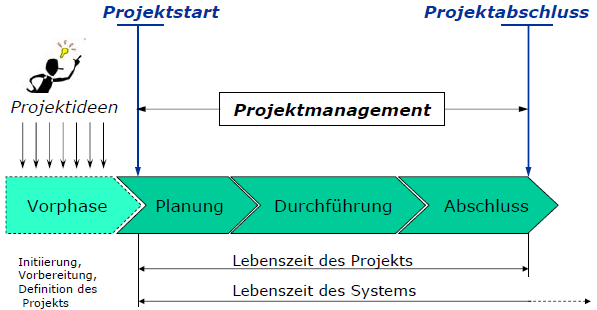
\includegraphics[width=\linewidth]{images/projektablauf.png}
\end{minipage}

\subsection{Projektphasen}
Verschiedene Teilprozesse können zeitlich parallel ablaufen. 
\subsubsection{Projektdefinition (Vorphase, Initiierung, Projektdefinition)}
\begin{itemize}
	\item Vorbereiten des Projektes
	\item evtl. Machbarkeitsstudie durchführen
	\item Ziele, Termine festlegen (Das Wichtigste eines Projektes)
	\item Grobe Aufwands- und Kostenschätzung, Projektorganisation festlegen
	\item Wird in formellen Projektauftrag festgehalten
\end{itemize}
	\begin{minipage}{9cm}
		\textbf{Projektauftrag} \\
		Der Projektauftrag ist ein schriftliches Dokument wo Ziele und Rahmenbedingungen festgehalten sind. Das Dokument wird vom Auftraggeber unterzeichnet, damit ist Existenz des Projektes formell bestätigt. \newline Die Ziele des Projektes sollten gemäss \textcolor{blue}{S.M.A.R.T.} formuliert sein.\newline
        {\small\textbf{ Häufige Bestandteile:}}
        \vspace{-0.3cm}
        \begin{multicols}{2}
            {\small
            \begin{itemize}
                \item Projektbezeichnung
                \item Auftraggeber
                \item Projektbeginn / -ende
                \item Kurzbeschreibung
                \item Projektergebnisse
                \item Projektbudget
                \item Projektleiter
                \item Terminvorgaben   
            \end{itemize}  }   
        \end{multicols}
	\end{minipage}
    \hfill
	\begin{minipage}{8.5cm}
		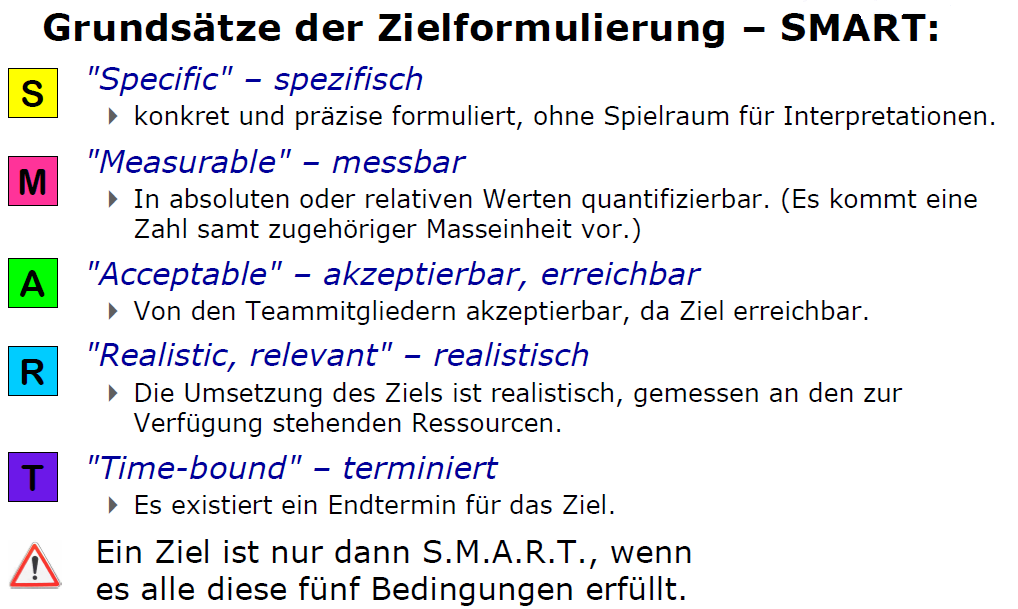
\includegraphics[width=\linewidth]{images/pmstart.png}
	\end{minipage}
\vspace{-0.5cm}	
\subsubsection{Projektplanung}
Als Voraussetzung zur Projektplanung gilt der erstellte Projektauftrag. Anschliessend findet das \textcolor{blue}{\textit{"Kick-Off-Meeting"}} statt. \newline Das \textit{"Kick-Off-Meeting"} gilt als \textcolor{blue}{offizieller Projektstart}., $\rightarrow$ \textbf{Hauptziel:} Alle sind arbeitsfähig!\\
Die Projektplanung ist das Wichtigste. Die Pläne werden periodisch überarbeitet da niemals alles nach Plan läuft. \newline 
$\rightarrow$ \textbf{Wichtig:} \textcolor{blue}{\textbf{Meilensteine}} setzen
\vspace{0.2cm}
\\
\begin{minipage}{10cm}
	\textbf{1. Projektstrukturplan (PSP)}
	\begin{itemize}
		\item Projekt in Teilprojekte zerlegen
		\item Kleinstmögliche Aufgaben sind Arbeitspakete
		\item Arbeitspakete sind \textcolor{blue}{phasenorientiert} (nach Zeitabschnitten) oder \textcolor{blue}{objektorientiert} (nach Komponenten) oder \textcolor{blue}{funktionsorientiert} (nach Ähnlichkeit der Aufgaben) aufgeteilt
		\item Pro Arbeitspaket wird eine Arbeitsbeschreibung erstellt
	\end{itemize} 	
\end{minipage}
\begin{minipage}{9cm}
	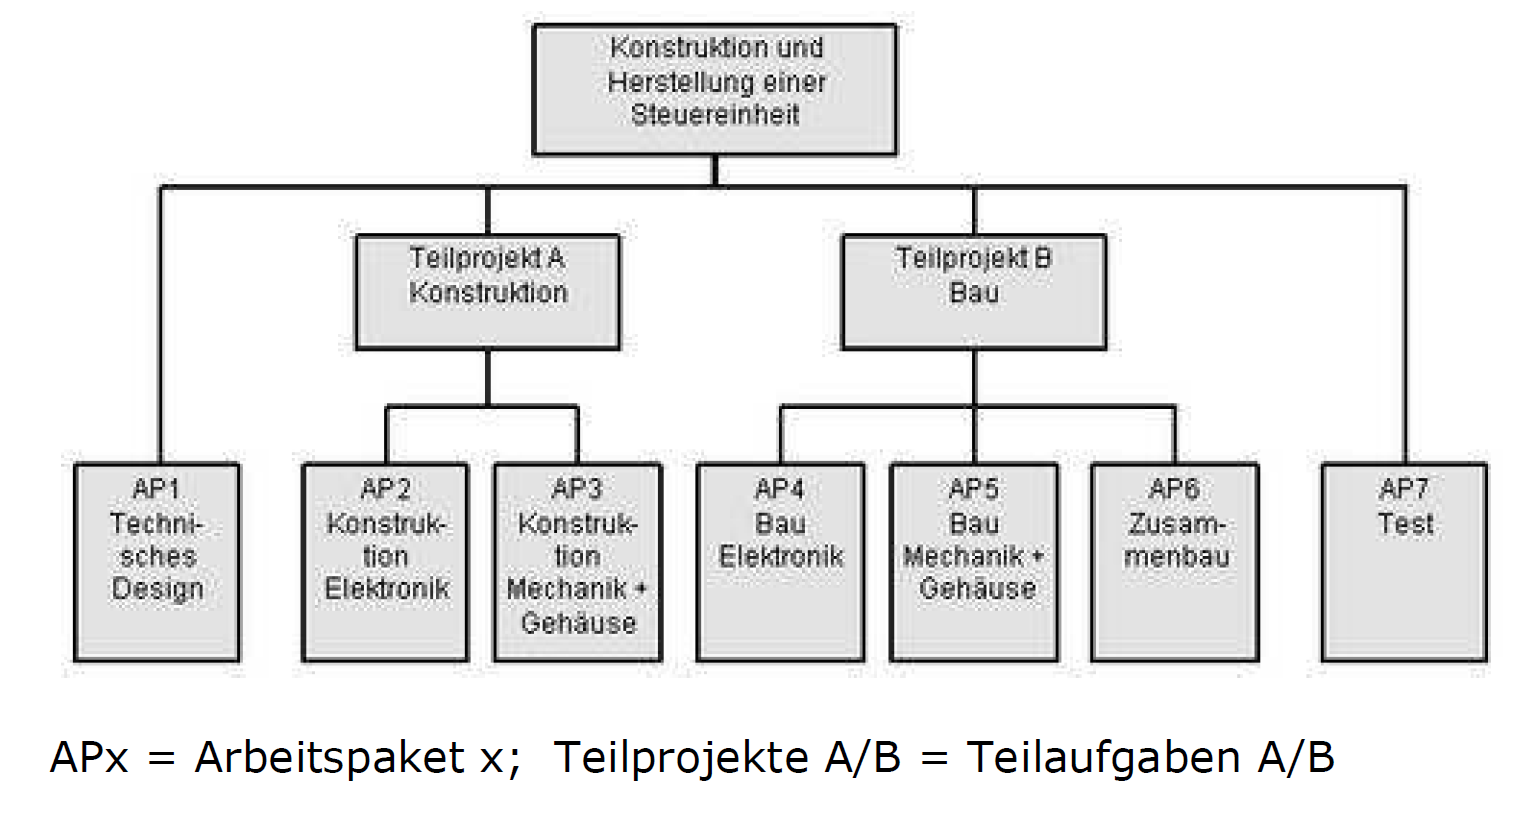
\includegraphics[width=9cm]{images/PSP.png}
\end{minipage}
\clearpage
\pagebreak

\textbf{Arbeitspakete}\\
\begin{center}
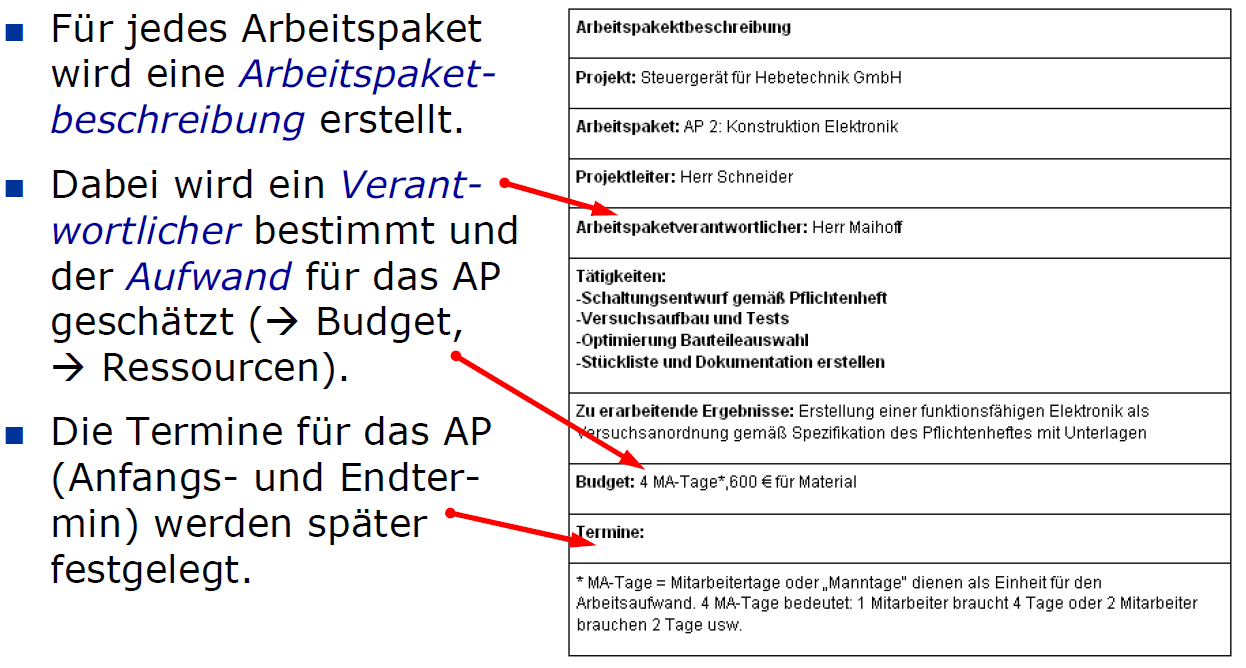
\includegraphics[width = 12cm]{images/arbeitsbeschreibung}
\end{center}
\vspace{-0.5cm}
\begin{multicols}{2}
\textbf{2. Projektablaufplan (PAP)} \\
Stellt die \textcolor{blue}{logische Abhängigkeiten} der Arbeitspakete dar. Dazu wird eine Vorgangsliste erstellt, welche die Abhängigkeiten zwischen den Arbeitspakete aufzeigt. \\
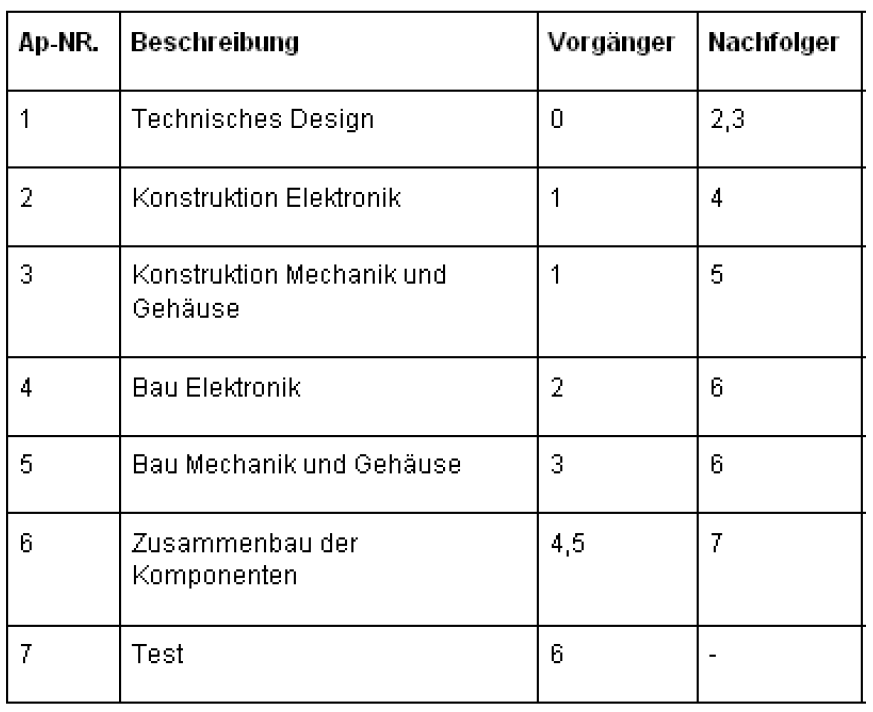
\includegraphics[width = 6cm]{images/ablaufsplan}
\end{multicols}

\renewcommand{\arraystretch}{1.2}
	\begin{tabular}{|l|l|l|}
		\hline \textbf{Abhängigkeit} & \textbf{Funktion} & \textbf{Bild} \\
		\hline Normalfolge & Nachfolger kann erst beginnen, wenn Vorgänger beendet ist & \tabbild[width=4cm]{images/normalfolge.png}\\
		\hline Anfangsfolge & Nachfolger kann erst beginnen, wenn Vorgänger begonnen hat &
		\tabbild[width=4cm]{images/anfangsfolge} \\
		\hline Endfolge & Nachfolger kann erst enden, wenn Vorgänger beendet ist &
		\tabbild[width=4cm]{images/endfolge.png} \\
		\hline Sprungfolge & Nachfolger kann erst enden wenn Vorgänger begonnen hat &
		\tabbild[width=4cm]{images/sprungfolge.png}\\
		\hline
	\end{tabular}\newline
\vspace{0.2cm}
\\
\\
\textbf{3. Projektterminplan}
\begin{itemize}
	\item Zuordnung von Terminen zu den Arbeitspaketen
	\item Festlegen der \textcolor{blue}{Meilensteine/Milestones} (= wichtige Termine)
    \begin{itemize}
    	\item Meilensteine sind Etappenziele welche zur Projektkontrolle dienen
    	\item Meilensteine sind so formuliert, dass \textit{"'Erfüllt"} oder \textit{" Nicht Erfüllt"} gilt
    	\item Meilensteine stehen am Ende jeder Projektphase    	
    \end{itemize}
	\item Projektterminplan wird aufgrund des PSP und PAP erstellt
\end{itemize}
	\begin{tabular}{l l l}
		 \textbf{Balkendiagramm} & \textbf{Netzplan} & \textbf{Microsoft Project} \\
		 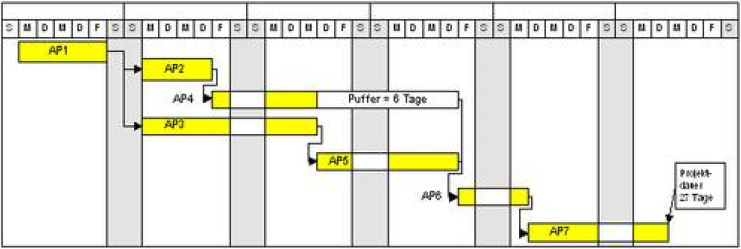
\includegraphics[width=6cm]{images/balkendiagramm} & 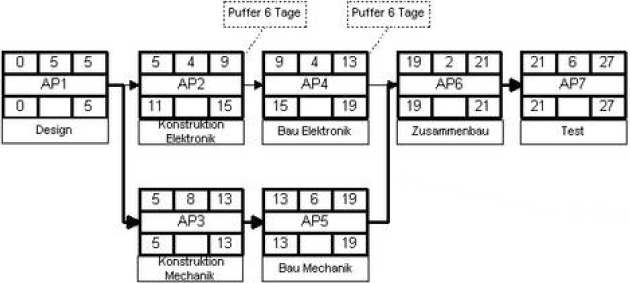
\includegraphics[width=6cm]{images/netzplan}	& 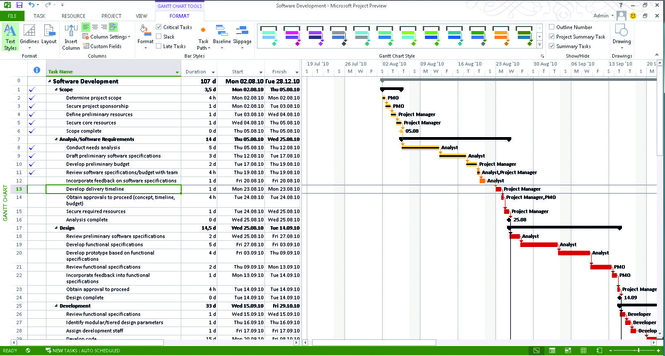
\includegraphics[width=6cm]{images/msproject}	 
	\end{tabular}
\clearpage

\textbf{3.1 Microsoft Project}\\
In MS Project wird immer von Task (Vorgang) gesprochen.\newline
MS Project hat als Grundlage das Balkendiagramm und die Netzplantechnik.\\
Wichtigster Zusammenhang: \textbf{Work = Duration $\cdot$ Units}\\
\begin{multicols}{2}
	\begin{itemize}
		\item \textbf{Einzelvorgang (Sub Task)} $\rightarrow$ Arbeitspaket
		\item \textbf{Sammelvorgang (Summary Task)} \newline $\rightarrow$ mehrere Vorgänge
		\item \textbf{Vorgang mit Dauer 0} $\rightarrow$ Meilenstein	
	\end{itemize}
	\begin{itemize}
		\item \textbf{Fixed Units} $\rightarrow$ Ressourcen = konstant
		\item \textbf{Fixed Work} $\rightarrow$ Arbeit = konstant
		\item \textbf{Fixed Duration} $\rightarrow$ Dauer = konstant
	\end{itemize}
\end{multicols}

\begin{tabular}{|l|l|l|}
	\hline \textbf{Work}& Arbeitsumfang & Einheit: Anzahl Personentage, Mannstunden\\
	\hline \textbf{Duration} & Zeitdauer & Einheit: Anzahl Stunden,Tage\\
	\hline \textbf{Units}& Intensität& Einheit: Angabe der Beteiligung in Prozent\\
	\hline
\end{tabular}\\\\
\textbf{4. Ressourcen- und Kapazitätsplan}\\
Die benötigten Ressourcen ermitteln und mit den Kapazitäten abstimmen. 
\\
\\
\textbf{5. Kosten- und Budgetplan}\\
Die Kosten für für die Ressourcen schätzen und Budget erstellen. 

\subsubsection{Projektdurchführung}
Die eigentliche Arbeit beginnt. Der Projektleiter hat die Aufgabe des Projekt-Controlling (to control $\rightarrow$ steuern).\\
\textcolor{blue}{Projekt-Controlling = Projektkontrolle + Projektsteuerung}
\renewcommand{\arraystretch}{1.2}
\begin{table}[h!]
	\begin{tabular}{|l|l|}
		\hline \textbf{Projektkontrolle} 	& Rechtzeitiges Feststellen von Abweichungen gegenüber dem geplanten \\ 
		& Soll-Ist-Vergleich\\
		\hline  \textbf{Projektsteuerung} 	& Massnahmen um Projekt bei Abweichungen wieder auf Zielkurs zu bringen. \\
		& Soll-Werte anpassen\\
		\hline
	\end{tabular}
\end{table}

\subsubsection{Projektabschluss}
\begin{itemize}
	\item Eigentliche Projektarbeit wurde erfolgreich abgeschlossen.
	\begin{itemize}
		\item Ziele sind erreicht
	\end{itemize}
	\item Formaler Abschluss des Projekts mit dem Auftraggeber:
	\begin{itemize}
		\item Projektpräsentation
		\item Projektabnahme, Übergabe, Entlastung des PL.
		\item Allfällige Nacharbeiten
	\end{itemize}
	\item Projektteam interner Abschluss
	\begin{itemize}
		\item Abschlussmeeting: Manöverkritik, \"{}Lessons learned\"{}
		\item Abschlussfeier
	\end{itemize}
\end{itemize}
\clearpage